% To make handouts: (eg)
% pdfnup --nup 2x2 --orient landscape --frame true --delta "1cm 1cm" --scale 0.9 lecture.pdf 
% except pdfnup isn't yet on the system at ECS... (I've asked for it).

%% BEAMER TUTORIAL:   http://www.math.umbc.edu/~rouben/beamer/quickstart.html


% remove/add "handout" to the following, to disable/enable presentation overlays
\documentclass[slidestop,compress,mathserif]{beamer}

\usepackage{multimedia}
\usepackage{amsfonts}
\usepackage[scaled]{helvet}
\setcounter{tocdepth}{2} % determines the depth to which tableofcontents goes

%% For lots of theme examples, see  http://www.hartwork.org/beamer-theme-matrix/
%\usetheme[height=8mm]{Boadilla}
\usetheme{Frankfurt}
\setbeamertemplate{items}[rectangle] 
\setbeamertemplate{blocks}[rounded][upper=black,lower=white,shadow=false]
%\usecolortheme{default} % default albatross crane beetle dove fly seagull wolverine beaver
\usecolortheme{lily} % for blocks: lily, orchid, rose... beaver
%\setbeamertemplate{navigation symbols}{} % gets rid of those silly navigations!

%\beamersetaveragebackground{black}
\setbeamercolor{alerted text}{fg=red}






% couple of handy things for my maths
\newcommand{\independent}{\protect\mathpalette{\protect\independenT}{\perp}}
\def\independenT#1#2{\mathrel{\rlap{$#1#2$}\mkern2mu{#1#2}}}
\newcommand{\dependent}{\not\independent}
\newcommand{\data}{\mathcal{D}}
\newcommand{\mat}[1]{\ensuremath{\mathbf{#1}}} % vectors/matrices, x,A,B etc.
\newcommand{\gmat}[1]{\mbox{\boldmath${#1}$}}  % vectors/matrices Greek symbols
\newcommand{\swrt}[2]{\frac{\partial #1}{\partial #2}} % partial derivative of single symbol
\newcommand{\bwrt}[1]{\frac{\partial}{\partial #1}} % partial derivative of something big
\newcommand{\bx}{\mat{x}}
\newcommand{\bh}{\mat{h}}
\newcommand{\bw}{\mat{w}}
\newcommand{\bv}{\mat{v}}
\newcommand{\by}{\mat{y}}
\newcommand{\bs}{\mat{s}}
\newcommand{\bt}{\mat{t}}
\newcommand{\bm}{\mat{m}}
\newcommand{\bX}{\mat{X}}
\newcommand{\bT}{\mat{T}}
\newcommand{\bW}{\mat{W}}
\newcommand{\bY}{\mat{Y}}

\newcommand{\real}{\mathbb{R}}
\newcommand{\reals}{\mathbb{R}}
\newcommand{\Expectation}{\mathbb{E}}
\newcommand{\expectation}{\mathbb{E}}
\newcommand{\obs}{\mathrm{obs}}
\newcommand{\half}{\mbox{\small $\frac{1}{2}$}}
\newcommand{\tinyhalf}{\mbox{\tiny $\frac{1}{2}$}}

%\renewenvironment{itemize}{\begin{dinglist}{96}}{\end{dinglist}}
\definecolor{MyBlue}{rgb}{0,0.2,0.85}
\definecolor{blue}{rgb}{0,0.08,0.45}
\definecolor{green}{rgb}{0,0.4,0.06}
\definecolor{lightgreen}{rgb}{0,0.8,0.12}
\definecolor{red}{rgb}{0.65,0.02,0.0}
\definecolor{lightblue}{rgb}{0.8,0.88,1}
\definecolor{example}{rgb}{1,1,0.7}
\definecolor{gray}{rgb}{.5,.5,.5}
\setbeamercolor{uppercol}{fg=white,bg=blue}
\setbeamercolor{lowercol}{fg=black,bg=lightblue}
\setbeamercolor{example}{fg=black,bg=example}
\renewcommand{\emph}{\color{MyBlue}}
\newcommand{\gray}{\color{gray}}
\newcommand{\blue}{\color{MyBlue}}
\newcommand{\red}{\color{red}}
\newcommand{\green}{\color{green}}
\newcommand{\lightgreen}{\color{lightgreen}}
\newcommand{\Line}[0]{\rule{0cm}{0cm}\\\hrule\rule{0cm}{0cm}}

\setlength{\parskip}{2mm plus 1mm minus 1mm}




\date{}

\title{Source finding by model comparison}
\author{Marcus Frean, Anna Friedlander, \\Melanie Johnston-Hollitt and Chris Hollitt}
\institute{Victoria University of Wellington \\ Wellington, New Zealand}

\begin{document}
\frame{
  \titlepage


}


\frame{\frametitle{}
NEED: detect very faint objects embedded in noise, robustly,
efficiently, with a minimum of manual tuning.

\begin{center}
\includegraphics[width=.9\textwidth]{./pics/flda_gs} 
\end{center}
}

\frame{\frametitle{}
\begin{center}
\includegraphics[width=.65\textwidth]{./pics/test} 
\end{center}
}


\frame{
      \includegraphics[width=.35\textwidth]{./pics/pics-555B}
      \pause \\
      \includegraphics[width=.35\textwidth]{./pics/pics-555-bin-eqwidth}
      \pause \\
      \includegraphics[width=.35\textwidth]{./pics/pics-555-bin-eqocc}
}



%% \frame{
%% ``Raw'' input: images as floats.

%% Standard approach : find a bright pixel, and ``grow'' / ``floodfill''
%% a region around it by including neighbours that seem brighter than
%% they should be under the background distribution.

%% {\it good as doesn't commit to some model of shape... good for
%% compact bright, not so good for diffuse, dim.}

%% {\em But robustly, efficiently, with a minimum of manual tuning? }

%% Our approach: discretize, identify a distribution (histogram)
%% corresponding to the ``background'', and search for regions
%% in the image that seem seem to come from a different distribution.

%% [Q:  what is the background distribution? Addressed elsewhere].
%% }



%% \section{smooth binning}
%% \frame{\frametitle{ways of binning}
%% \begin{itemize}
%% \item equal width?
%% \item equal occupancy?
%% \item exponentially increasing..?
%% \end{itemize}

%% It's not obvious which is to be prefered.

%% And even if we knew ``the best'', the bin borders cause artifacts: they don't model anything ``real''.
%% }


\frame{\frametitle{dirichlet borders}
There are no ``correct'' borders, so we generate {\em lots of them}. 

Use the Dirichlet distribution to make the bin borders:
\begin{center}
\begin{tabular}{lcr} $\alpha=(1,1,1)\;\;\;\;\;\;\;\;\;\;\;\;\;\;\;$ &$\alpha=(10,10,10)$ &$\;\;\;\;\;\;\;\;\;\;\;\;\;\alpha=(2,5,20)$ \end{tabular}\\
    \includegraphics[width=.99\textwidth]{./pics/simplex}
\pause \\
    \includegraphics[width=.99\textwidth]{./pics/dirichlet_draws_1}
\end{center}

%So instead of a pixel being attributed to a single bin, we get a distribution.

%(show a couple of histograms  - talk about how Dir gives sample in the simplex, which we can interpret as a normalised histogram of probs.)

% (say how parameters of Dirichlet enable us to make different sorts of histograms....)
% (hyperparameters  $\alpha$ are like ``pseudo counts'').

%Say: {\em Representing that we are uncertain} about the borders removes the {\em edge effects}.
}

\frame{\frametitle{dirichlet borders}
There are no ``correct'' borders: so we generate {\em lots of them}. 

Use the Dirichlet distribution to make the bin borders:
\begin{center}
\begin{tabular}{lcr} $\alpha=(1,1,1)\;\;\;\;\;\;\;\;\;\;\;\;\;\;\;$ &$\alpha=(10,10,10)$ &$\;\;\;\;\;\;\;\;\;\;\;\;\;\alpha=(2,5,20)$ \end{tabular}\\
    \includegraphics[width=.99\textwidth]{./pics/simplex} \\
    \includegraphics[width=.99\textwidth]{./pics/dirichlet_draws_2}
\end{center}
}

\frame{\frametitle{dirichlet borders}
There are no ``correct'' borders: so we generate {\em lots of them}. 

Use the Dirichlet distribution to make the bin borders:
\begin{center}
\begin{tabular}{lcr} $\alpha=(1,1,1)\;\;\;\;\;\;\;\;\;\;\;\;\;\;\;$ &$\alpha=(10,10,10)$ &$\;\;\;\;\;\;\;\;\;\;\;\;\;\alpha=(2,5,20)$ \end{tabular}\\
    \includegraphics[width=.99\textwidth]{./pics/simplex} \\
    \includegraphics[width=.99\textwidth]{./pics/dirichlet_draws_3}
\end{center}
}

\frame{\frametitle{dirichlet borders}
There are no ``correct'' borders: we generate {\em lots of them}. 

Use the Dirichlet distribution to make the bin borders:
\begin{center}
\begin{tabular}{lcr} $\alpha=(1,1,1)\;\;\;\;\;\;\;\;\;\;\;\;\;\;\;$ &$\alpha=(10,10,10)$ &$\;\;\;\;\;\;\;\;\;\;\;\;\;\alpha=(2,5,20)$ \end{tabular}\\
    \includegraphics[width=.99\textwidth]{./pics/simplex} \\
    \includegraphics[width=.33\textwidth]{./pics/stacked_a}
    \includegraphics[width=.33\textwidth]{./pics/stacked_b}
    \includegraphics[width=.33\textwidth]{./pics/stacked_c}
\end{center}
}


\frame{\frametitle{so we don't have to believe in just one binning scheme}
\vspace{-1.5em}
  \begin{columns}
   \begin{column}[]{0.5\textwidth} % 1st column
       \begin{block}{$\sim$ Equal bins}
             \includegraphics[width=.9\textwidth]{./pics/test_DirBins_s1_a100}
       \end{block}
    \end{column}
    \pause
   \begin{column}[]{0.5\textwidth} % 1st column
       \begin{block}{$\sim$ Exponential bins}
             \includegraphics[width=.9\textwidth]{./pics/test_DirBins_s1p3_a100}
       \end{block}
    \end{column}
  \end{columns}
}


\frame{
      \includegraphics[width=.35\textwidth]{./pics/pics-555A}
}


\frame{
      \includegraphics[width=.35\textwidth]{./pics/pics-555B}
      \pause \\
      \includegraphics[width=.35\textwidth]{./pics/pics-555-bin-eqwidth}
      \hspace{1cm} \pause
      \includegraphics[width=.35\textwidth]{./pics/pics-555-bin-eqwidth-dirichlet}
      \pause \\
      \includegraphics[width=.35\textwidth]{./pics/pics-555-bin-eqocc}
      \hspace{1cm} \pause
      \includegraphics[width=.35\textwidth]{./pics/pics-555-bin-eqocc-dirichlet}
}



\section{scoring a region}
\frame{\frametitle{How to score a region in an image?}
\begin{center}
\includegraphics[width=.9\textwidth]{./pics/flda_gs_box} 
\end{center}
}


\subsection{compare multinomial distributions?}
\frame{\frametitle{How to score a region in an image?}

figure out the {\bf categorical} distributions typical of pixels from background and {\color{blue}source},  and compare the likelihoods under a multinomial model...
  \begin{columns}
    \begin{column}[]{0.5\textwidth} % 1st column
        \begin{block}{}
        
\includegraphics[scale=.55]{./pics/Mult} 
         \end{block}
    \end{column}
    \pause
    \begin{column}[]{0.5\textwidth} % 1st column
        \begin{block}{}
        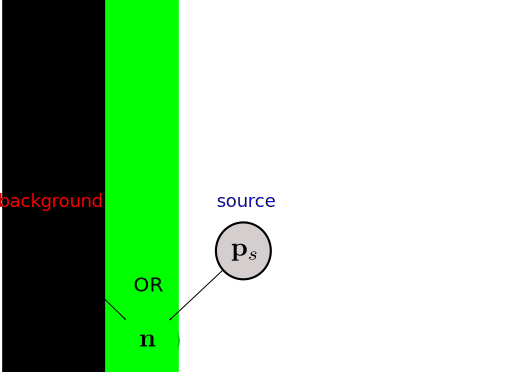
\includegraphics[scale=.55]{./pics/MultRatio} 
        \pause
\[ \text{score} = \log \frac{P(\mathbf{n} \mid  \text{\color{blue}source})}{P(\mathbf{n} \mid  \text{\color{red}background})} \]
         \end{block}
    \end{column}
  \end{columns}

}



\frame{\frametitle{}

One can imagine such a model (histogram) for {\color{red}background}, but 
\begin{itemize}
\item<2->\alert<2>{all {\color{blue}sources} are different - we should not commit to look for ``typical'' sources}
\item<3->\alert<3>{small region versus large region? Big region has more evidence: this {\it should} matter, but it won't.}
\end{itemize}

\Line

\begin{itemize}
\item<4->\alert<4>{
Ah! We could treat the background distribution as a (frequentist) null hypothesis to be rejected, or}
\item<5->\alert<5>{
do something sensible}
\end{itemize}

}


\subsection{Dirichlet-multinomial distribution}

\frame{\frametitle{The Dirichlet-multinomial distribution}
...a compound distribution, where the parameters
of a categorical distribution are drawn from a Dirichlet distribution with parameters
$\boldsymbol\alpha = \alpha_1 .. \alpha_K$.
  \begin{columns}
    \begin{column}[]{0.3\textwidth} % 1st column
    \begin{block}{}
    
\includegraphics[scale=.55]{./pics/DirMult} 
      \end{block}
    \end{column}
    \begin{column}[]{0.7\textwidth} % 1st column
    \begin{block}{}
\pause
We can integrate out \textbf{p} {\color{blue}analytically} $\longrightarrow$ evidence:
\begin{align*}
P(\textbf{n}\mid \alpha) &= \frac{\Gamma(A)}{\Gamma(N+A)} \prod_k \frac{\Gamma(n_k+\alpha_k)}{\Gamma(\alpha_k)}   
%\\\text{where} \;\;\;\;\;\;\;\;\;\;\;\; A &= \sum_k \alpha_k, \;\text{and} \;N = \sum_k n_k
\end{align*}
{\color{gray}\small (No MCMC required)}
      \end{block}
    \end{column}
\end{columns}
}

\frame{\frametitle{the Bayes factor}
\vspace{-1em}
  \begin{columns}
    \begin{column}[]{0.4\textwidth} % 1st column
    \begin{block}{}
 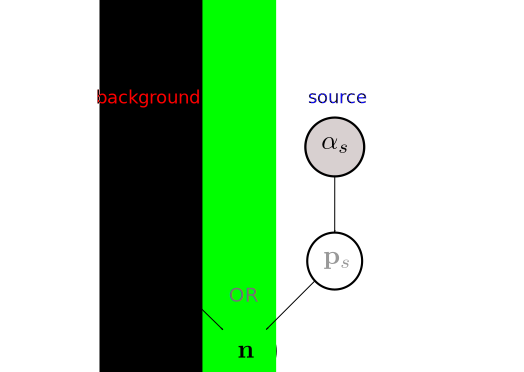
\includegraphics[scale=.6]{./pics/DirMultRatio} 
      \end{block}
    \end{column}
    \begin{column}[]{0.6\textwidth} % 1st column
    \begin{block}{}
\pause
\vspace{-1em}
\begin{align*}
\text{score} &= \log \frac{P(S \mid \mathbf{n} )}{P(B \mid \mathbf{n} )} \\
%\text{Score} 
&= \log \frac{P(\textbf{n} \mid  S)}{P(\textbf{n} \mid  B)} \;\; + \; 
\log \frac{P(S)}{P(B)}
\end{align*}
\begin{itemize}
\pause
\item {\color{red}background}: lots of evidence - typical by definition: we used the overall counts as the hyperparameters $\alpha_B$
\pause
\item {\color{blue}source}: much less evidence for ``typical'': we set all $\alpha_S$ to 1
\end{itemize}
      \end{block}
    \end{column}
\end{columns}

\pause
A score of zero means we're right on the fence for this region.
}

%% \frame{\frametitle{Bayes factor}
%% The ratio of posterior probabilities for the two models indicates how
%% well a particular region fails to conform to what's expected to come
%% from a ``background'' region. 

%% The log of this ratio is a reasonable ``score'':
%% \begin{align*}
%% \text{score} &= \log \frac{P(S \mid \mathbf{n} )}{P(B \mid \mathbf{n} )} \\
%% %\text{Score} 
%% &= \log \frac{P(\textbf{n} \mid  S)}{P(\textbf{n} \mid  B)} \;\; + \; 
%% \log \frac{P(S)}{P(B)}
%% \end{align*}

%% Can fairly compare a model with large
%% $\alpha$'s (ie. a well established prior distribution) with one having
%% small $\alpha$'s (ie. a poorly established prior distribution, since weird pixel distributions are rare).

%% %The second term is a constant.
%% }


\section{region boundaries}
\subsection{region boundaries}
%% \frame{
%% \includegraphics[width=1.08\textwidth]{./pics/hard-to-soft-borders-hard}
%% %\vspace{1em}
%% \\\pause
%% \includegraphics[width=1.08\textwidth]{./pics/hard-to-soft-borders-soft}
%% %\includegraphics[width=0.25\textwidth]{./pics/hard-soft-borders}
%% }

%% \frame{
%% \includegraphics[width=1.08\textwidth]{./pics/hard-to-soft-borders-soft}
%% \vspace{1em}
%% \includegraphics[width=0.25\textwidth]{./pics/hard-soft-borders}
%% }
\frame{\frametitle{soft boundaries $\longrightarrow$ partial counts}
\vspace{1em}
\includegraphics[width=0.8\textwidth]{./pics/hard-soft-borders}
}

%% \frame{\frametitle{soft region boundaries}
%% With an all-or-nothing definition of ``region'', a pixel is either in or out.

%% But this seems unreasonable: we used a Gaussian-shaped kernel instead:
%% \begin{center}
%%     \includegraphics[width=0.55\textwidth]{./pics/hard-soft-borders}
%% \end{center}
%% }



\frame{\frametitle{1-D simulated data}
\begin{center}
    \includegraphics[width=.95\textwidth]{./pics/1d-score-egs2A}
\end{center}

(uses Dirichlet-generated, $\sim$equal occupancy bins)

%Note that the source at 446 has lower variance than is typical of the image.
}


\frame{\frametitle{1-D simulated data}
\begin{center}
    \includegraphics[width=.95\textwidth]{./pics/1d-score-egs2B}
\end{center}

(uses Dirichlet-generated, $\sim$equal occupancy bins)

%Note that the source at 446 has lower variance than is typical of the image.
}


%% \section{1D examples}
%% \frame{\frametitle{1-D simulated data}
%% \begin{center}  \includegraphics[width=\textwidth]{./pics/DMR_333_width_K15_nostreams} \end{center}
%% }
%% \frame{\frametitle{1-D simulated data}
%% \begin{center}  \includegraphics[width=\textwidth]{./pics/DMR_333_width_K15} \end{center}
%% }
%% \frame{\frametitle{1-D simulated data}
%% \begin{center}  \includegraphics[width=\textwidth]{./pics/DMR_333_eqocc_K15} \end{center}
%% }


\frame{\frametitle{1-D simulated data (eg 2)}
\begin{center}  \includegraphics[width=1.1\textwidth]{./pics/DMR_555_width_K15} \end{center}
}
\frame{\frametitle{1-D simulated data (eg 2)}
\begin{center}  \includegraphics[width=1.1\textwidth]{./pics/DMR_555_eqocc_K15} \end{center}
}


\frame{\frametitle{1-D simulated data (eg 3)}
\begin{center}  \includegraphics[width=1.1\textwidth]{./pics/DMR_888_width_K15} \end{center}
}
\frame{\frametitle{1-D simulated data (eg 3)}
\begin{center}  \includegraphics[width=1.1\textwidth]{./pics/DMR_888_eqocc_K15} \end{center}
}



%% \frame{
%% To evaluate the ideas on ``data'' for which we know ground truth,  we used skewed, generalised Gaussian functions
%% \begin{center}
%%     \includegraphics[width=.75\textwidth]{./pics/skewed_gen_gaussian_curves}
%% \end{center}
%% }

%% \frame{\frametitle{1-D ``real'' data}
%% \begin{center}
%%     \includegraphics[width=.65\textwidth]{./pics/1d-comp-binning}
%% \end{center}

%% DMR score on a one dimensional “slice” of an astronomical image (ATLSB survey region A at 50' resolution). Results using equal occupancy (top left), equal width (top
%% right), Dirichlet equal occupancy (bottom left), and Dirichlet equal width
%% (bottom right) histogram binning strategies.

%% For this example peaks in gradient best correspond to the actual
%% peaks in data in the case of the Dirichlet equal width binning strategy.
%% }


\section{2D examples}
\frame{\frametitle{DMR score on 2-D simulated data}
\begin{center}
    \includegraphics[width=\textwidth]{./pics/eqdir-binned-score} 
\end{center}

}


\section{iterative removal}
\frame{\frametitle{iterative removal of sources}
\begin{center}
\includegraphics[width=\textwidth]{./pics/progbinned}
\end{center}

At each round of gradient ascent, a source is removed, and the bin borders and $\alpha^B$ vector recalculated.

With each round, new sources are revealed that were previously hidden in ``background'' bins.
}

\subsection{real example}
\frame{\frametitle{comparisons}
    \includegraphics[width=.65\textwidth]{./pics/comparisons} 

%A section of one of the CDFS test-windows.

%% Top right: sources identified by BLOBCAT (raw, unprocessed output). 

%% Bottom left: sources in the ground-truth catalogue

%% bottom right: those identified by our algorithm

%% ie. found in the ground truth catalogue, plus
%% \begin{itemize}
%% \item part of a low brightness source (radio galaxy tail; pink ring). 
%% \item has correctly split sources that catalogue identified as one (blue ring)
%% \end{itemize}

}


%=================================================================

  %% \begin{beamerboxesrounded}[upper=uppercol,lower=lowercol,shadow=true]
  %%   {thing}
  %%   wordsy wordsy
  %% \end{beamerboxesrounded}

\frame{

\begin{center}
    \includegraphics[width=\textwidth]{./pics/1d-score-egs2B}
\end{center}

}


\end{document}
